What follows is mostly from From Jang \etal (2005) \cite{jalk05}.

The non-conforming finite element space is defined based on the 
reference cubic element $Q_l$ on $[-1,1]^3$ :
\[
Q_l = \text{Span} \left\{ 1, r, s, t, \theta_l(r)-\theta_l(s), \theta_l(r)-\theta_l(t) \right\}
\qquad l=1,2
\]
with\footnote{Douglas \etal \cite{doss99}, Eq.~2.20} 
\begin{eqnarray}
\theta_1(r) &=& r^2-\frac53r^4  \nn\\
\theta_2(r) &=& r^2-\frac{25}{6} r^4 + \frac72 r^6 
\end{eqnarray}
The dimension of $Q_l$ is six and the $\theta_l$ functions are as follows:
\begin{center}
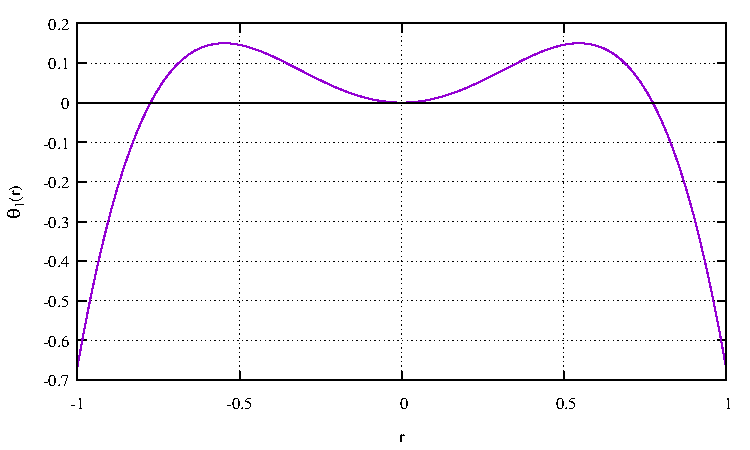
\includegraphics[width=7cm]{images/dssy/theta1}
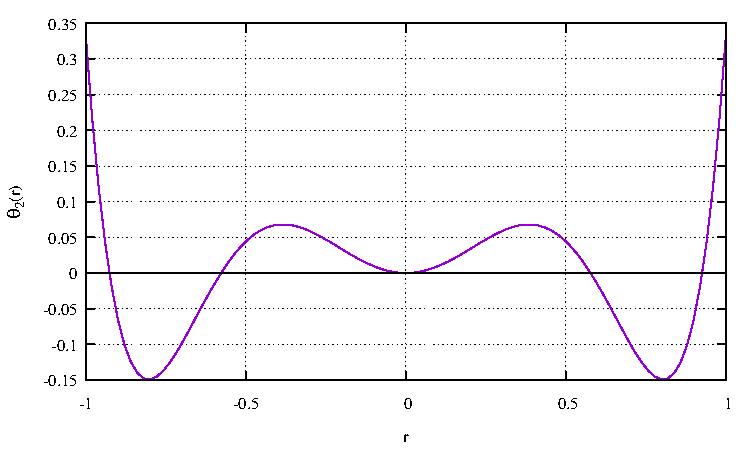
\includegraphics[width=7cm]{images/dssy/theta2}\\
{\captionfont Representation of functions $\theta_1$ (left) and 
$\theta_2$ (right).} 
\end{center}
We have:
\begin{itemize}
\item $\theta_1(r=-1)=\theta_1(r=+1)=-\frac23$, $\theta_1(r=0)=0$ 
\item $\theta_2(r=-1)=\theta_2(r=+1)=\frac13$, $\theta_2(r=0)=0$ 
\end{itemize}
These functions have the property that their average on an edge is zero:
\begin{eqnarray}
\frac{1}{1-(-1)}\int_{-1}^{+1} \theta_1(r) dr 
&=& \frac{1}{2}\int_{-1}^{+1} \left( r^2-\frac53r^4  \right) dr \nn\\
&=& \frac12 \left( \frac23 - \frac53 \frac25 \right) \nn\\
&=& 0 \nn\\
\frac{1}{1-(-1)}\int_{-1}^{+1} \theta_2(r) dr 
&=& \frac{1}{2}\int_{-1}^{+1} \left( r^2-\frac{25}{6} r^4 + \frac72 r^6  \right) dr \nn\\
&=& \frac{1}{2} \left( \frac23 -\frac{25}{6} \frac25 + \frac72 \frac{2}{7}  \right) dr \nn\\
&=& 0 \nn
\end{eqnarray}
The element has 6 nodes that are located at the face centres of a cube or a brick.
The pointwise continuity between interfacing elements is guaranteed only at the face centers,
so the field quantities are not conforming along the interface \cite{jalk05}.

\begin{flushright} {\tiny {\color{gray} (tikz\_dssy3D.tex)}} \end{flushright}
%~~~~~~~~~~~~~~~~~~~~~~~~~~~~~~~~~~~~~~~~~~~~~~~~~~~~~~~~~~~~~~~~~~~~~~~~~~~~~~~~~~~~~~~~~~~~~~~~~~

\begin{center}
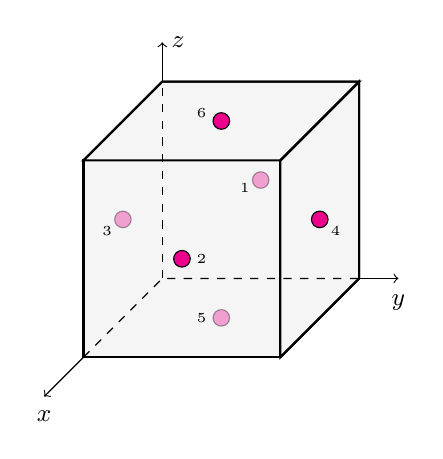
\begin{tikzpicture}

%\draw[step=1cm,gray,very thin] (0,0) grid (8,8); %background grid

\draw[thick,fill=gray!8] (5,1) -- (7.5,1) -- (7.5,3.5) -- (5,3.5) -- cycle;
\draw[thick,fill=gray!8] (7.5,1) -- (8.5,2) -- (8.5,4.5) -- (7.5,3.5) -- cycle;
\draw[thick,fill=gray!8] (5,3.5) -- (7.5,3.5) -- (8.5,4.5) -- (6,4.5) -- cycle;
\draw[thick] (5,3.5) -- (6,4.5) -- (8.5,4.5) -- (8.5,2) -- (7.5,1);
\draw[thick] (7.5,3.5) -- (8.5,4.5) ;
\draw[dashed] (5,1) -- (6,2) -- (8.5,2) ;\draw[dashed] (6,2) -- (6,4.5);


\draw[black,fill=magenta,opacity=0.35] (5.5,2.75)   circle (3pt);
\draw[black,fill=magenta] (8,2.75)   circle (3pt);
\draw[black,fill=magenta,opacity=0.35] (6.75,1.5)   circle (3pt);
\draw[black,fill=magenta] (6.75,4)   circle (3pt);
\draw[black,fill=magenta] (6.25,2.25)   circle (3pt);
\draw[black,fill=magenta,opacity=0.35] (7.25,3.25)   circle (3pt);

\node[] at (7.05,3.15) {\tiny 1};
\node[] at (6.5,2.25) {\tiny 2};
\node[] at (5.3,2.6) {\tiny 3};
\node[] at (8.2,2.6) {\tiny 4};
\node[] at (6.5,1.5) {\tiny 5};
\node[] at (6.5,4.1) {\tiny 6};

\draw[->] (5,1)--(4.5,0.5);
\draw[->] (8.5,2)--(9,2);
\draw[->] (6,4.5)--(6,5);

\node[] at (4.5,0.25) {\small $x$};
\node[] at (9,1.7) {\small $y$};
\node[] at (6.2,5) {\small $z$};

\end{tikzpicture}
\end{center}


(axis should actually be in the middle of the cube!)

The six nodes of the reference element are 
\[
\begin{array}{c|ccc}
\hline
\vec{r}_1 &-1 &0 &0 \\
\vec{r}_2 &+1 &0 &0 \\
\vec{r}_3 &0 &-1 &0 \\
\vec{r}_4 &0 &+ &0 \\
\vec{r}_5 &0 &0 &-1 \\
\vec{r}_6 &0 &0 &+1 \\
\hline
\end{array}
\]
and their corresponding basis functions:
\begin{eqnarray}
N_1^{(l)}(r,s,t) &=&  \frac16 - \frac12 r + \frac{1}{6\theta_l(1)}(2\theta_l(r)-\theta_l(s)-\theta_l(t))  \nn\\
N_2^{(l)}(r,s,t) &=&  \frac16 + \frac12 r + \frac{1}{6\theta_l(1)}(2\theta_l(r)-\theta_l(s)-\theta_l(t))  \nn\\
N_3^{(l)}(r,s,t) &=&  \frac16 - \frac12 s + \frac{1}{6\theta_l(1)}(2\theta_l(s)-\theta_l(t)-\theta_l(r))  \nn\\
N_4^{(l)}(r,s,t) &=&  \frac16 + \frac12 s + \frac{1}{6\theta_l(1)}(2\theta_l(s)-\theta_l(t)-\theta_l(r))  \nn\\
N_5^{(l)}(r,s,t) &=&  \frac16 - \frac12 t + \frac{1}{6\theta_l(1)}(2\theta_l(t)-\theta_l(r)-\theta_l(s))  \nn\\
N_6^{(l)}(r,s,t) &=&  \frac16 + \frac12 t + \frac{1}{6\theta_l(1)}(2\theta_l(t)-\theta_l(r)-\theta_l(s))  
\end{eqnarray}
These basis functions are also in \cite{doss99}.
We can easily verify that $\sum_i N_i(r,s,t)=1$ and that $N_i(\vec{r}_j)=\delta_{ij}$:
\begin{eqnarray}
N_1^{(l)}(r_1,s_1,t_1) 
&=& \frac16 - \frac12 (-1) + \frac{1}{6\theta_l(1)}(2\theta_l(-1)-\theta_l(0) -\theta_l(0)) = 1 \nn\\ 
N_1^{(l)}(r_2,s_2,t_2) 
&=& \frac16 - \frac12 (+1) + \frac{1}{6\theta_l(1)}(2\theta_l(+1)-\theta_l(0) -\theta_l(0)) = 0 \nn\\ 
N_1^{(l)}(r_3,s_3,t_3) 
&=& \frac16 - \frac12 (0)  + \frac{1}{6\theta_l(1)}(2\theta_l(0) -\theta_l(-1)-\theta_l(0)) = 0 \nn\\ 
N_1^{(l)}(r_4,s_4,t_4) 
&=& \frac16 - \frac12 (0)  + \frac{1}{6\theta_l(1)}(2\theta_l(0) -\theta_l(+1)-\theta_l(0)) = 0\nn\\ 
N_1^{(l)}(r_5,s_5,t_5) 
&=& \frac16 - \frac12 (0)  + \frac{1}{6\theta_l(1)}(2\theta_l(0) -\theta_l(0) -\theta_l(-1)) = 0\nn\\ 
N_1^{(l)}(r_6,s_6,t_6) 
&=& \frac16 - \frac12 (0)  + \frac{1}{6\theta_l(1)}(2\theta_l(0) -\theta_l(0) -\theta_l(+1))  = 0\nn
\end{eqnarray}
etc ...


\begin{eqnarray}
\partial_r N_1^{(l)}(r,s,t) &=&  - \frac12  + \frac{1}{3\theta_l(1)}\theta_l'(r)  \nn\\
\partial_r N_2^{(l)}(r,s,t) &=&  + \frac12  + \frac{1}{3\theta_l(1)}\theta_l'(r)  \nn\\
\partial_r N_3^{(l)}(r,s,t) &=&  -\frac{1}{6\theta_l(1)}\theta_l'(r)  \nn\\
\partial_r N_4^{(l)}(r,s,t) &=&  -\frac{1}{6\theta_l(1)}\theta_l'(r)  \nn\\
\partial_r N_5^{(l)}(r,s,t) &=&  -\frac{1}{6\theta_l(1)}\theta_l'(r)  \nn\\
\partial_r N_6^{(l)}(r,s,t) &=&  -\frac{1}{6\theta_l(1)}\theta_l'(r)  
\end{eqnarray}

\begin{eqnarray}
\partial_s N_1^{(l)}(r,s,t) &=&   -\frac{1}{6\theta_l(1)}\theta_l'(s) \nn\\
\partial_s N_2^{(l)}(r,s,t) &=&   -\frac{1}{6\theta_l(1)}\theta_l'(s) \nn\\
\partial_s N_3^{(l)}(r,s,t) &=& - \frac12  + \frac{1}{3\theta_l(1)}\theta_l'(s)  \nn\\
\partial_s N_4^{(l)}(r,s,t) &=& + \frac12  + \frac{1}{3\theta_l(1)}\theta_l'(s)  \nn\\
\partial_s N_5^{(l)}(r,s,t) &=&   \frac{1}{6\theta_l(1)}\theta_l'(s)  \nn\\
\partial_s N_6^{(l)}(r,s,t) &=&   \frac{1}{6\theta_l(1)}\theta_l'(s)  
\end{eqnarray}

\begin{eqnarray}
\partial_t N_1^{(l)}(r,s,t) &=& - \frac{1}{6\theta_l(1)}\theta_l(t)  \nn\\
\partial_t N_2^{(l)}(r,s,t) &=& - \frac{1}{6\theta_l(1)}\theta_l(t)  \nn\\
\partial_t N_3^{(l)}(r,s,t) &=& - \frac{1}{6\theta_l(1)}\theta_l(t)  \nn\\
\partial_t N_4^{(l)}(r,s,t) &=& - \frac{1}{6\theta_l(1)}\theta_l(t)  \nn\\
\partial_t N_5^{(l)}(r,s,t) &=& - \frac12 t + \frac{1}{3\theta_l(1)}\theta_l(t)  \nn\\
\partial_t N_6^{(l)}(r,s,t) &=& + \frac12 t + \frac{1}{3\theta_l(1)}\theta_l(t)  
\end{eqnarray}

\Literature: Douglas \etal (1999) \cite{doss99}, 
